% Importar librerias
\documentclass{IEEEtran}
\usepackage[utf8]{inputenc}%modifica las ñ y las tíldes para no colocar el cod ascii.
\usepackage[total={18cm,21cm},top=2cm, left=2cm, bottom=3cm]{geometry}
\usepackage[dvips]{graphicx}
\usepackage{multirow}
\usepackage{listings}
\usepackage[spanish, english]{babel}
\usepackage[x11names,table]{xcolor}
\usepackage{amsmath,amssymb,amsfonts,latexsym,cancel}%Funciones especiales para matemáticas
\usepackage{float} % Fijar posicion
\usepackage[hidelinks]{hyperref}
\newcommand\numberthis{\addtocounter{equation}{1}\tag{\theequation}}

\usepackage{algorithm}
\usepackage[noend]{algpseudocode}

% Precompilar PDF
\lstset{numbers=left, numberstyle=\scriptsize, numbersep=5pt, language=python, frame=single, fontadjust, basicstyle=\scriptsize, frameround=tttt, stepnumber=1, keywordstyle=\color{cyan}, showtabs=false, tab=\rightarrowfill} \renewcommand*\thelstnumber{\oldstylenums{\the\value{lstnumber}}}
\makeatletter
\def\contentsname{Indice}
\def\listfigurename{Lista de Figuras}
\def\listtablename{Lista de Tablas}
\def\refname{Referencias}
\def\indexname{Indice de Términos}
\def\figurename{Fig.}
\@IEEEcompsocconfonly{\def\figurename{Figura} \def\tablename{Tabla}}
\def\partname{Parte}
\def\appendixname{Apéndice}
\def\abstractname{Abstract}
\def\IEEEkeywordsname{Palabras Claves}
\def\IEEEproofname{Demostración}
\makeatother
\ifCLASSOPTIONcompsoc
\else
\fi
\ifCLASSINFOpdf
\else
\fi
\providecommand{\PSforPDF}[1]{#1}

% Metodos
\newcommand\MYhyperrefoptions{bookmarks=true,bookmarksnumbered=true,
pdfpagemode={UseOutlines},plainpages=false,pdfpagelabels=true,
colorlinks=true,linkcolor={black},citecolor={black},pagecolor={black},
urlcolor={black},
pdftitle={ALGO_Lab1},
pdfsubject={Typesetting},
pdfauthor={Santiago},
pdfkeywords={incremental, insertionSort}}

% Aquí comienza el documento
\title{
	Laboratorio 2
}
\author{
    Santiago Álvarez Sepúlveda, ~\IEEEmembership{\url{saalvarezse@unal.edu.co}, Cód:~25481031}\\
    Universidad Nacional de Colombia, Sede Bogotá
}

\markboth{
	Algoritmos, Laboratorio II, 9~Septiembre~2018
}{B \MakeLowercase{\textit{et al.}}: IEEE.cls para Journals}

% Aquí comienza el contenido del documento
\begin{document}
\maketitle

\IEEEpeerreviewmaketitle
\IEEEtitleabstractindextext
\IEEEpeerreviewmaketitle

\section{Problema I}
Usando la Figura \ref{fig1} como modelo, ilustre la operación de Insertion Sort en el arreglo $A = {31, 41, 59, 26, 41, 58}$.
    
    \begin{figure}[H]
    \centering
    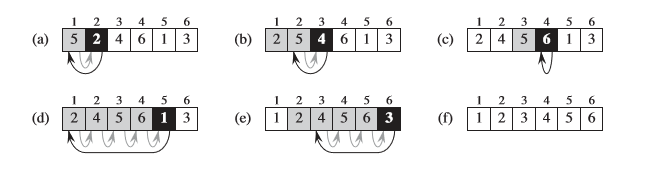
\includegraphics[width=0.5\textwidth]{img/fig1}
    \caption{Ilustración del algoritmo Insertion Sort}
    \label{fig1}
    \end{figure}

Siguiendo las instrucciones del algoritmo Insertion Sort para el arreglo especificado en el enunciado 1, se tiene el siguiente resultado:

    \begin{figure}[H]
    \centering
    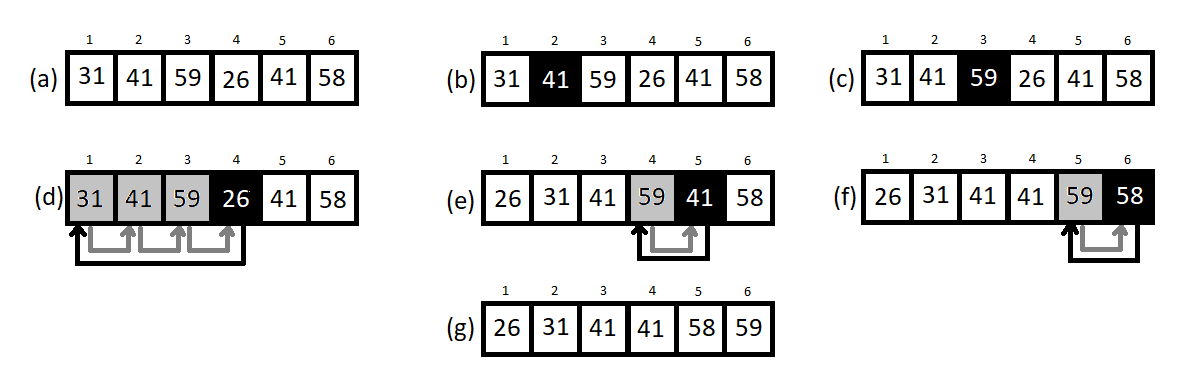
\includegraphics[width=0.5\textwidth]{img/fig2}
    \caption{Ilustración del algoritmo Insertion Sort para el arreglo del enunciado del problema I.}
    \label{fig2}
    \end{figure}
    
En la anterior figura se observa el proceso desde el arreglo inicial (Figura.\ref{fig2}.a), hasta el arreglo resultante (Figura.\ref{fig2}.g).
\section{Problema II}
Reescriba el procedimiento Insertion Sort para ordenar de manera descendiente y no en orden ascendente.

Se requiere un algoritmo que ordene un arreglo de tamaño $n$ por la técnica incremental de Insertion Sort. Modificando la condición del bucle \textit{While} del pseudocódigo del algoritmo para ordenar de manera ascendente, de forma que la condición ahora sea $i > 0$ and $A[i] < key$, entonces se van a desplazar los elementos menores que el elemento actual hacia la derecha, posicionando los elementos mayores a la izquierda del arreglo, es decir al comienzo.

\begin{algorithm}[H]
    \caption{Insertion Sort Descendiente}\label{alg:isort_desc}
    \begin{algorithmic}[1]
        \Procedure{InsertionSort}{$A$}
            \For{$j=2$ to $A$.length}
                \State $key = A[j]$
                \State $i = j-1$
                \While{$i > 0$ and $A[i] < key$}
                    \State $A[i+1] = A[i]$
                    \State $i = i-1$
                \EndWhile\label{isort_while}
                \State $A[i+1] = key$
            \EndFor\label{isort_for}
        \EndProcedure
    \end{algorithmic}
\end{algorithm}
\section{Problema III}
Considere el \textbf{problema de búsqueda}:
    
\textbf{Entrada:} Una secuencia de $n$ enteros $A = {a_1, a_2, ..., a_n}$ y un valor $v$.

\textbf{Salida:} Un índice $i$ tal que $v = A[i]$ o el valor especial \textit{NIL} si $v$ no existe en $A$.

Escriba un pseudocódigo para el algoritmo de \textbf{búsqueda lineal}, el cual recorre la secuencia buscando a $v$. Usando un bucle invariante pruebe que su algoritmo es correcto. Asegure que su bucle satisface las tres propiedades necesarias.

\begin{algorithm}[H]
    \caption{Linear Search}\label{alg:linear_search}
    \begin{algorithmic}[1]
        \Procedure{LinearSearch}{$A, v$}
            \State $key = NIL$
            \For{$j=1$ to $A$.length}
                \If{$A[j] = v$}
                    \State $key = j$
                \EndIf\label{linear_search_if}
            \EndFor\label{isort_for}
            \Return $key$
        \EndProcedure
    \end{algorithmic}
\end{algorithm}

\subsection{Inicialización}
Se debe demostrar que nuestro bucle invariante contiene el subconjunto $A[1, ..., j-1]$. Al inicializar la rutina, nuestro bucle invariante consiste de el elemento $NIL$, el cual retornaremos en el caso que no exista $v$ en el arreglo $A$. Esto demuestra que el bucle invariante se mantiene antes de iniciar la primera iteración del ciclo \textit{for} del algoritmo.

\subsection{Mantenimiento}
Cada iteración del algoritmo mantiene el bucle invariante ya que este va a cambiar su valor almacenado cuando se encuentre el elemento $v$
 en el arreglo $A$. De esta manera vemos que si se conserva el subconjunto de $A$ durante todas las iteraciones del algoritmo.
 
\subsection{Terminación}
Vemos que al terminar las iteraciones el ciclo \textit{for} del algoritmo, $j$ va a tener el valor $(n+1)$, una posición del arreglo que no es posible acceder. Por esta razón en este punto de la ejecución no se bisca indexar de nuevo una posición del arreglo con este índice, sino retorna el valor inicializado de la posición de $v$ en $A$, o $NIL$ en su defecto.
\section{Problema IV}
Considere el problema de sumar dos números enteros binarios de $n$ bits, almacenados en dos arreglos de $n$ elementos $A$ y $B$. La suma de los dos enteros debería ser almacenada en forma binaria en un arreglo de $(n+1)$ elementos $C$. Desarrolle el problema formalmente y escriba pseudocódigo para sumar estos dos números. 

\begin{algorithm}[H]
    \caption{Suma Binaria}\label{alg:linear_search}
    \begin{algorithmic}[1]
        \Procedure{BinarySum}{$A, B, n$}
            \State $C = zeros(n+1)$
            \While{$n > 0$}
                \State $C[n+1] = (A[n] \mathbin{\oplus} B[n]) \mathbin{\oplus} C[n+1]$
                \State $C[n] = (A[n] \land (B[n] \lor C[n])) \lor (B[n] \land C[n])$
                \State $n--$
            \EndWhile
            \Return $C$
        \EndProcedure
    \end{algorithmic}
\end{algorithm}

\subsection{Inicialización}
El anterior pseudocódigo asume que se tienen dos arreglos de bits $A$ y $B$ de tamaño $n$. Se inicializa con ceros un arreglo para almacenar el resultado de la suma $C$ de tamaño $(n+1)$. Así se garantiza que se reserva memoria suficiente para almacenar el resultado final.

\subsection{Mantenimiento}
En cada iteración del ciclo \textit{While} del algoritmo estamos utilizando el subarreglo $C[n, n+1]$ y $A[n], B[n]$ los cuales existen para cada valor de $n$ puesto que este valor no puede tomar valores menores a $1$, posición inicial de todos los arreglos.
 
\subsection{Terminación}
Ya que se ha impuesto un decremento al parámetro $n$ y una condición que haga que no se ejecuten más operaciones sobre elementos de los arreglos iniciales cuando este parámetro tenga un valor menor a $1$, es decir que se van a realizar n veces las iteraciones en el ciclo \textit{While} y al ser $n = 0$ se culminará la ejecución.

\end{document}